%----------------------------------------------------------------------------------------

\documentclass[a4paper,10pt]{article} % Uses article class in A4 format

%----------------------------------------------------------------------------------------
%	FORMATTING
%----------------------------------------------------------------------------------------

\setlength{\parskip}{0pt}
\setlength{\parindent}{0pt}
\setlength{\voffset}{-15pt}

%----------------------------------------------------------------------------------------
%	PACKAGES AND OTHER DOCUMENT CONFIGURATIONS
%----------------------------------------------------------------------------------------

\usepackage[a4paper, margin=2.5cm]{geometry} % Sets margin to 2.5cm for A4 Paper
\usepackage[onehalfspacing]{setspace} % Sets Spacing to 1.5

\usepackage[T1]{fontenc} % Use European encoding
\usepackage[utf8]{inputenc} % Use UTF-8 encoding
\usepackage{charter} % Use the Charter font
\usepackage{microtype} % Slightly tweak font spacing for aesthetics

\usepackage[english]{babel} % Language hyphenation and typographical rules

\usepackage{amsthm, amsmath, amssymb} % Mathematical typesetting
\usepackage{marvosym, wasysym} % More symbols
\usepackage{float} % Improved interface for floating objects
\usepackage[final, colorlinks = true, 
            linkcolor = black, 
            citecolor = black,
            urlcolor = black]{hyperref} % For hyperlinks in the PDF
\usepackage{graphicx, multicol} % Enhanced support for graphics
\usepackage{xcolor} % Driver-independent color extensions
\usepackage{rotating} % Rotation tools
\usepackage{listings, style/lstlisting} % Environment for non-formatted code, !uses style file!
\usepackage{pseudocode} % Environment for specifying algorithms in a natural way
\usepackage{style/avm} % Environment for f-structures, !uses style file!
\usepackage{booktabs} % Enhances quality of tables

\usepackage{tikz-qtree} % Easy tree drawing tool
\tikzset{every tree node/.style={align=center,anchor=north},
         level distance=2cm} % Configuration for q-trees
\usepackage{style/btree} % Configuration for b-trees and b+-trees, !uses style file!

\usepackage{titlesec} % Allows customization of titles
\renewcommand\thesection{\arabic{section}.} % Arabic numerals for the sections
\titleformat{\section}{\large}{\thesection}{1em}{}
\renewcommand\thesubsection{\alph{subsection})} % Alphabetic numerals for subsections
\titleformat{\subsection}{\large}{\thesubsection}{1em}{}
\renewcommand\thesubsubsection{\roman{subsubsection}.} % Roman numbering for subsubsections
\titleformat{\subsubsection}{\large}{\thesubsubsection}{1em}{}

\usepackage[all]{nowidow} % Removes widows

\usepackage[backend=biber,style=numeric,
            sorting=nyt, natbib=true]{biblatex} % Complete reimplementation of bibliographic facilities
\addbibresource{main.bib}
\usepackage{csquotes} % Context sensitive quotation facilities

\usepackage[yyyymmdd]{datetime} % Uses YEAR-MONTH-DAY format for dates
\renewcommand{\dateseparator}{-} % Sets dateseparator to '-'

\usepackage{fancyhdr} % Headers and footers
\pagestyle{fancy} % All pages have headers and footers
\fancyhead{}\renewcommand{\headrulewidth}{0pt} % Blank out the default header
\fancyfoot[L]{\textsc{Robin Worreby}} % Custom footer text
\fancyfoot[C]{} % Custom footer text
\fancyfoot[R]{\thepage} % Custom footer text

\newcommand{\note}[1]{\marginpar{\scriptsize \textcolor{red}{#1}}} % Enables comments in red on margin
\usepackage[shortlabels]{enumitem}
\usepackage{minted}
\usemintedstyle{friendly}
\usepackage[bf]{caption}
%----------------------------------------------------------------------------------------

\begin{document}

%----------------------------------------------------------------------------------------
%	TITLE SECTION
%----------------------------------------------------------------------------------------

\title{template_assignment} % Article title
\fancyhead[C]{}
\begin{minipage}{0.295\textwidth} % Left side of title section
\raggedright
HPCSE1\\ % Your lecture or course
\footnotesize % Authors text size
%\hfill\\ % Uncomment if right minipage has more lines
Robin Worreby, 16-921-298 % Your name, your matriculation number
\medskip\hrule
\end{minipage}
\begin{minipage}{0.4\textwidth} % Center of title section
\centering 
\large % Title text size
Exercise 06\\ % Assignment title and number
\normalsize % Subtitle text size
MPI IO, Hybrid MPI + OpenMP,\\
ADI scheme, and PSE method % Assignment subtitle
\end{minipage}
\begin{minipage}{0.295\textwidth} % Right side of title section
\raggedleft
\today\\ % Date
\footnotesize % Email text size
%\hfill\\ % Uncomment if left minipage has more lines
rworreby@student.ethz.ch% Your email
\medskip\hrule
\end{minipage}

%----------------------------------------------------------------------------------------
%	ARTICLE CONTENTS
%----------------------------------------------------------------------------------------

\setcounter{section}{0}

\section{Diffusion: Parallel I/O}

\begin{enumerate}[a)]
\setcounter{enumi}{0}
\item 
Figure \ref{fig:parallel_io} shows the written data from the parallel MPI IO code and Figure \ref{fig:euler} show how the modules on EULER were loaded.
\begin{figure}[h!]
  \centering
  \begin{minipage}[t]{0.8\textwidth}
    
\includegraphics[width=\textwidth]{plots/dump_parallel.png}
    \caption{Plot of the data written by the parallel MPI IO function. Parameters: $D = 1, L = 2, N = 1024, ranks = 16$}
    \label{fig:parallel_io}
  \end{minipage}
  \hfill
  \begin{minipage}[t]{0.8\textwidth}
    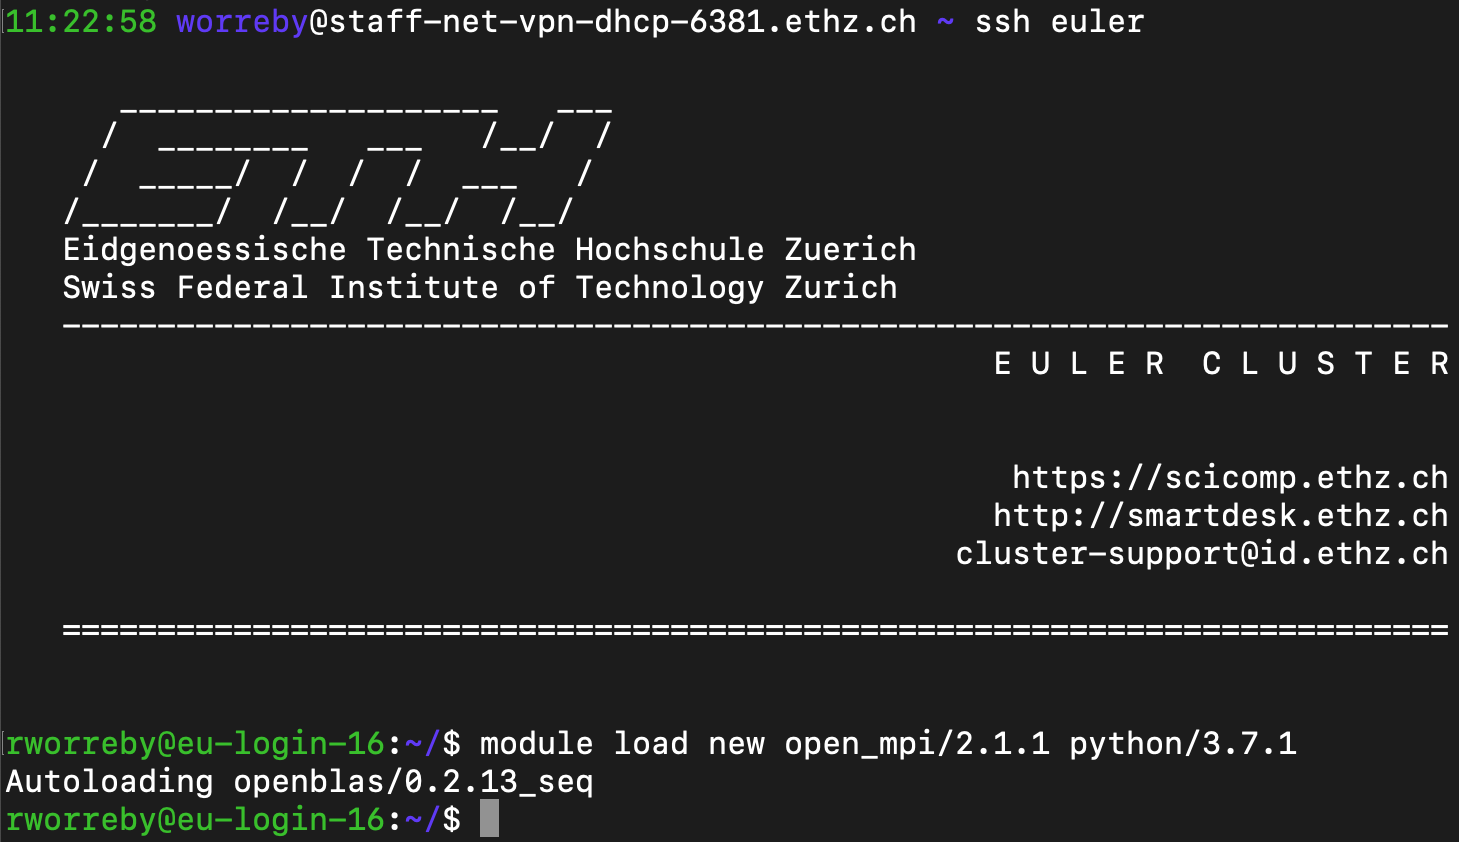
\includegraphics[width=1\textwidth]{plots/euler_module_loading.png}
    \caption{Screenshot showing the loading of the modules on EULER.}
    \label{fig:euler}
  \end{minipage}
\end{figure}
    
\item
We use $16$ ranks to check the performance of our parallel MPI IO implementation. When plotting the results, as seen in Figure \ref{fig:parallel_scaling}, we can see that the parallel version demonstrates a better scaling performance. For a gridsize $N \times N$ with $N = 6144$ we can see that the execution time of the file write is roughly $3x$ lower for the parallel version. As we use $16$ ranks our max achievable speedup is $S = 16$. We assume that the reason for not reaching this is because of the overhead from the MPI operations, like calculating the file pointer locations and opening the files on all ranks. Additionally, the amount of data we're writing is still rather small and we expect the gap to further increase as the data size increases. The presumed bottleneck in the sequential version is the sending of the data to the main rank, which is omitted for the parallel version. Another thing to note is that for very small sizes the sequential implementation outperforms the parallel version. This is, however, no surprise as the overhead described above is computationally more expensive than sending the data to the main rank for small data.

\begin{figure}[h!]
  \centering
  \begin{minipage}[t]{0.8\textwidth}
    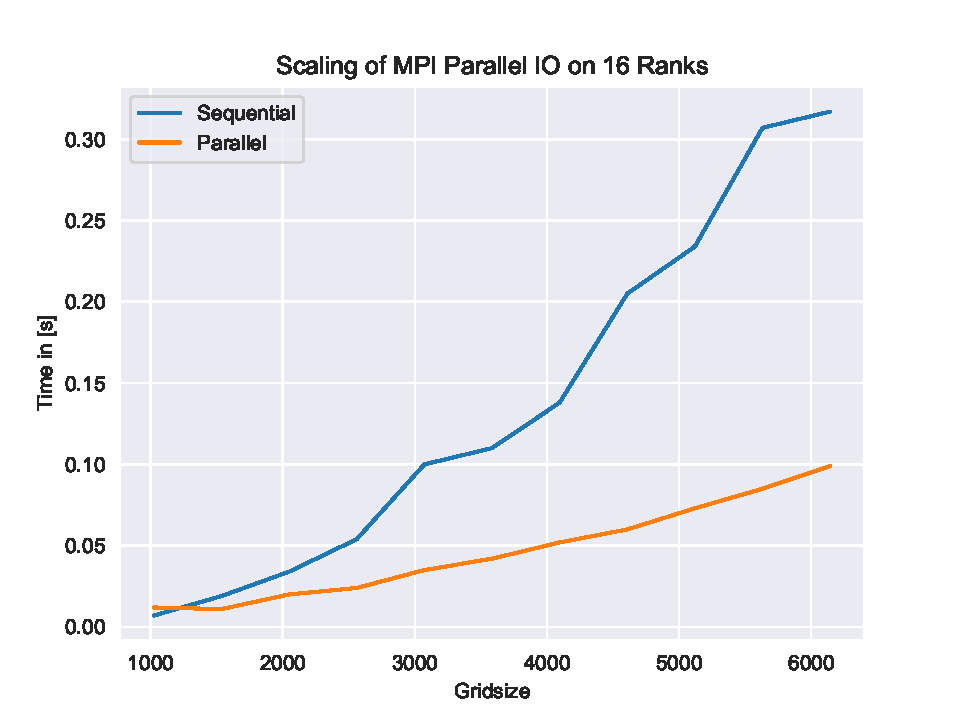
\includegraphics[width=\textwidth]{plots/parallel_io_scaling.pdf}
    \caption{Plot of the parallel MPI IO scaling.}
    \label{fig:parallel_scaling}
  \end{minipage}
\end{figure}

\end{enumerate}
\bigskip
%----------------------------------------------------------------------------------------
%	REFERENCE LIST
%----------------------------------------------------------------------------------------

\printbibliography

%----------------------------------------------------------------------------------------

\end{document}

